\documentclass[12pt]{article}

\usepackage[utf8x]{inputenc} % Включаем поддержку UTF8  
\usepackage[russian]{babel}  % Включаем пакет для поддержки русского языка  
\usepackage{hyperref}        % Для гиперссылок

% Математика
\usepackage{amsmath,amsfonts,amssymb,amsthm,mathtools} % AMS
\usepackage{icomma}
\usepackage{mathrsfs}

\usepackage{xcolor}

% Прога
\usepackage{etoolbox}
\usepackage{listings}

\definecolor{codegreen}{rgb}{0,0.6,0}
\definecolor{codegray}{rgb}{0.5,0.5,0.5}
\definecolor{codepurple}{rgb}{0.58,0,0.82}
\definecolor{backcolour}{rgb}{0.95,0.95,0.92}

\lstdefinestyle{mystyle}{
	backgroundcolor=\color{backcolour},   
	commentstyle=\color{codegreen},
	keywordstyle=\color{magenta},
	numberstyle=\tiny\color{codegray},
	stringstyle=\color{codepurple},
	basicstyle=\ttfamily\footnotesize,
	breakatwhitespace=false,         
	breaklines=true,                 
	captionpos=b,                    
	keepspaces=true,                 
	numbers=left,                    
	numbersep=5pt,                  
	showspaces=false,                
	showstringspaces=false,
	showtabs=false,                  
	tabsize=2
}

\lstset{style=mystyle}

% Цвета
\usepackage{xcolor}

% Картинки
\usepackage{graphicx}
\graphicspath{ {./images/} }

\usepackage{tikzsymbols}

% Работа с таблицами
\usepackage{array,tabularx,tabulary,booktabs} % Дополнительная работа с таблицами
\usepackage{longtable}  % Длинные таблицы
\usepackage{multirow} % Слияние строк в таблице

% Нумерованные списки
\usepackage[shortlabels]{enumitem} % Разные лейблы

% Текст
\usepackage[normalem]{ulem}  % для зачеркивания текста

\newtheorem{property}{Свойство}
\newtheorem{consequence}{Следствие}[property]

\begin{document}
	
	\thispagestyle{empty}
	\begin{center}
		\textbf{ПРАВИТЕЛЬСТВО РОССИЙСКОЙ ФЕДЕРАЦИИ}
		
		\vspace{5ex}
		
		\textbf{Федеральное государственное автономное образовательное учреждение \\ высшего образования \\ <<Национальный исследовательский университет \\ <<Высшая школа экономики>>}
	\end{center}
	\vspace{5ex}
	
	\begin{center}
		Московский институт электроники и математики им. А.Н. Тихонова  
		
		\vspace{5ex}
		
		Департамент прикладной математики
		
		\vspace{10ex}
		\textbf{Отчёт \\ по лабораторной работе A4.1 \\ по курсу <<Компьютерный практикум>> \\ Задание № 13}
		\vspace{7ex}
		
	\end{center}
	
	\begin{center} 
		\begin{tabular}{| p{0.3\linewidth}| p{0.3\linewidth}| p{0.3\linewidth}|}
			\hline	
			ФИО студента & Номер группы & Дата \\  \hline
			& & \\  
			Кейер Александр \newline Петрович & БПМ-231 & \today \\  
			& & \\  \hline		
		\end{tabular}
	\end{center}
	
	\begin{center}
		\vspace{3ex}
		
		\vfill
		
		\normalsize
		
		\textbf{Москва, 2024}
	\end{center}
	
	\newpage
	
	%---------------------------------------------------------------------------------
	
	\section*{Задание}
	
	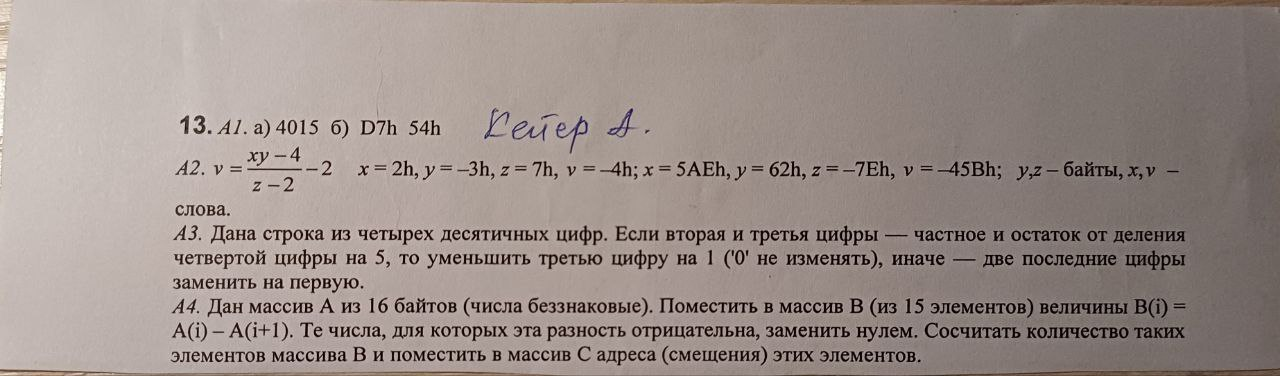
\includegraphics[width=400pt]{variant_13.jpg}
	
	Дана строка из четырех десятичных цифр. Если вторая и третья цифры -- частное и остаток от деления четвертой цифры на 5, то уменьшить третью цифру на 1 ('0' не изменять), иначе -- две последние цифры заменить на первую.
	
	\newpage
	
	%---------------------------------------------------------------------------------
	
	\section*{Решение}\addcontentsline{toc}{section}{}
	
	\begin{lstlisting}[language=C]
#include <stdio.h> // Input/output library.
#include <string.h> // String library for special function: strlen etc.

int testCounter = 1;

void printUnsignedCharArray(unsigned char arr[16], int ALength) {
	if (ALength == 0) {
		return;
	}
	
	printf("%d", arr[0]);
	
	for (int i = 1; i < ALength; i++) {
		printf(", %d", arr[i]);
	}
	
	printf("\n");
}

void printIntArray(int arr[15], int ALength) {
	if (ALength == 0) {
		return;
	}
	
	printf("%d", arr[0]);
	
	for (int i = 1; i < ALength; i++) {
		printf(", %d", arr[i]);
	}
	
	printf("\n");
}

void test(unsigned char A[16]) {
	printf("Test %d.\n", testCounter++);
	printf("A: ");
	printUnsignedCharArray(A, 16);
	
	unsigned char B[15] = {0};
	int C[15] = {0};
	
	int CLength = 0;
	
	__asm__ (
	"mov esi, %1;      \n"
	"lea edi, %2;      \n"
	"lea ebx, %3;      \n"
	
	"mov ecx, 15;      \n"
	
	"loop_start:           \n"
	"mov al, [esi];    \n"
	"inc esi;           \n"
	"mov dl, [esi];    \n"
	
	"sub al, dl;      \n"
	"js negative;      \n"
	
	"mov [edi], al;     \n"
	"jmp loop_continue \n"
	
	"negative:    \n"
	"mov [ebx], edi; \n"
	
	"inc ebx; \n"
	"inc %0; \n"
	
	"jmp loop_continue \n"
	
	"loop_continue: \n"
	"inc edi;           \n"
	"dec ecx;          \n"
	
	"cmp ecx, 0;         \n"
	"jne loop_start     \n"
	
	: "=m" (CLength)
	: "m" (A), "m" (B), "m" (C)
	: "esi", "edi", "eax", "ebx", "ecx", "edx"
	);
	
	printf("B: ");
	printUnsignedCharArray(B, 15);
	
	printf("C: ");
	printIntArray(C, CLength);
}

int main() {
	// Test 1.
	unsigned char A[16] = {13, 12, 13, 15, 1, 10, 9, 8, 7, 6, 5, 4, 3, 2, 1, 0};
	
	test(A);
	
	return 0;
}
	\end{lstlisting}
	
	\newpage
	
	%---------------------------------------------------------------------------------
	
	\section*{Тесты}\addcontentsline{toc}{section}{}
	
	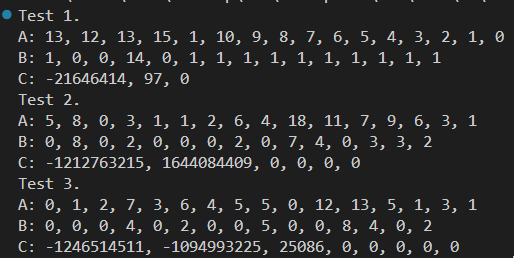
\includegraphics[width=400pt]{tests.png}
	
	Как видим, для массива B программа отрабатывает отлично, но возникают какие-то проблемы с массивом C.
	
\end{document}
